\documentclass[1p]{elsarticle_modified}
%\bibliographystyle{elsarticle-num}

%\usepackage[colorlinks]{hyperref}
%\usepackage{abbrmath_seonhwa} %\Abb, \Ascr, \Acal ,\Abf, \Afrak
\usepackage{amsfonts}
\usepackage{amssymb}
\usepackage{amsmath}
\usepackage{amsthm}
\usepackage{scalefnt}
\usepackage{amsbsy}
\usepackage{kotex}
\usepackage{caption}
\usepackage{subfig}
\usepackage{color}
\usepackage{graphicx}
\usepackage{xcolor} %% white, black, red, green, blue, cyan, magenta, yellow
\usepackage{float}
\usepackage{setspace}
\usepackage{hyperref}

\usepackage{tikz}
\usetikzlibrary{arrows}

\usepackage{multirow}
\usepackage{array} % fixed length table
\usepackage{hhline}

%%%%%%%%%%%%%%%%%%%%%
\makeatletter
\renewcommand*\env@matrix[1][\arraystretch]{%
	\edef\arraystretch{#1}%
	\hskip -\arraycolsep
	\let\@ifnextchar\new@ifnextchar
	\array{*\c@MaxMatrixCols c}}
\makeatother %https://tex.stackexchange.com/questions/14071/how-can-i-increase-the-line-spacing-in-a-matrix
%%%%%%%%%%%%%%%

\usepackage[normalem]{ulem}

\newcommand{\msout}[1]{\ifmmode\text{\sout{\ensuremath{#1}}}\else\sout{#1}\fi}
%SOURCE: \msout is \stkout macro in https://tex.stackexchange.com/questions/20609/strikeout-in-math-mode

\newcommand{\cancel}[1]{
	\ifmmode
	{\color{red}\msout{#1}}
	\else
	{\color{red}\sout{#1}}
	\fi
}

\newcommand{\add}[1]{
	{\color{blue}\uwave{#1}}
}

\newcommand{\replace}[2]{
	\ifmmode
	{\color{red}\msout{#1}}{\color{blue}\uwave{#2}}
	\else
	{\color{red}\sout{#1}}{\color{blue}\uwave{#2}}
	\fi
}

\newcommand{\Sol}{\mathcal{S}} %segment
\newcommand{\D}{D} %diagram
\newcommand{\A}{\mathcal{A}} %arc


%%%%%%%%%%%%%%%%%%%%%%%%%%%%%5 test

\def\sl{\operatorname{\textup{SL}}(2,\Cbb)}
\def\psl{\operatorname{\textup{PSL}}(2,\Cbb)}
\def\quan{\mkern 1mu \triangleright \mkern 1mu}

\theoremstyle{definition}
\newtheorem{thm}{Theorem}[section]
\newtheorem{prop}[thm]{Proposition}
\newtheorem{lem}[thm]{Lemma}
\newtheorem{ques}[thm]{Question}
\newtheorem{cor}[thm]{Corollary}
\newtheorem{defn}[thm]{Definition}
\newtheorem{exam}[thm]{Example}
\newtheorem{rmk}[thm]{Remark}
\newtheorem{alg}[thm]{Algorithm}

\newcommand{\I}{\sqrt{-1}}
\begin{document}

%\begin{frontmatter}
%
%\title{Boundary parabolic representations of knots up to 8 crossings}
%
%%% Group authors per affiliation:
%\author{Yunhi Cho} 
%\address{Department of Mathematics, University of Seoul, Seoul, Korea}
%\ead{yhcho@uos.ac.kr}
%
%
%\author{Seonhwa Kim} %\fnref{s_kim}}
%\address{Center for Geometry and Physics, Institute for Basic Science, Pohang, 37673, Korea}
%\ead{ryeona17@ibs.re.kr}
%
%\author{Hyuk Kim}
%\address{Department of Mathematical Sciences, Seoul National University, Seoul 08826, Korea}
%\ead{hyukkim@snu.ac.kr}
%
%\author{Seokbeom Yoon}
%\address{Department of Mathematical Sciences, Seoul National University, Seoul, 08826,  Korea}
%\ead{sbyoon15@snu.ac.kr}
%
%\begin{abstract}
%We find all boundary parabolic representation of knots up to 8 crossings.
%
%\end{abstract}
%\begin{keyword}
%    \MSC[2010] 57M25 
%\end{keyword}
%
%\end{frontmatter}

%\linenumbers
%\tableofcontents
%
\newcommand\colored[1]{\textcolor{white}{\rule[-0.35ex]{0.8em}{1.4ex}}\kern-0.8em\color{red} #1}%
%\newcommand\colored[1]{\textcolor{white}{ #1}\kern-2.17ex	\textcolor{white}{ #1}\kern-1.81ex	\textcolor{white}{ #1}\kern-2.15ex\color{red}#1	}

{\Large $\underline{12a_{0528}~(K12a_{0528})}$}

\setlength{\tabcolsep}{10pt}
\renewcommand{\arraystretch}{1.6}
\vspace{1cm}\begin{tabular}{m{100pt}>{\centering\arraybackslash}m{274pt}}
\multirow{5}{120pt}{
	\centering
	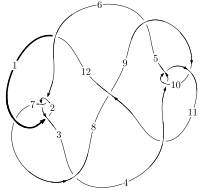
\includegraphics[width=112pt]{../../../GIT/diagram.site/Diagrams/png/1329_12a_0528.png}\\
\ \ \ A knot diagram\footnotemark}&
\allowdisplaybreaks
\textbf{Linearized knot diagam} \\
\cline{2-2}
 &
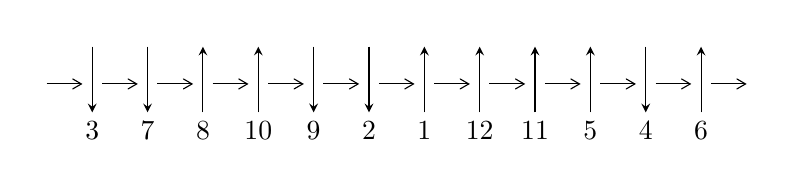
\begin{tikzpicture}[x=20pt, y=17pt]
	% nodes
	\node (C0) at (0, 0) {};
	\node (C1) at (1, 0) {};
	\node (C1U) at (1, +1) {};
	\node (C1D) at (1, -1) {3};

	\node (C2) at (2, 0) {};
	\node (C2U) at (2, +1) {};
	\node (C2D) at (2, -1) {7};

	\node (C3) at (3, 0) {};
	\node (C3U) at (3, +1) {};
	\node (C3D) at (3, -1) {8};

	\node (C4) at (4, 0) {};
	\node (C4U) at (4, +1) {};
	\node (C4D) at (4, -1) {10};

	\node (C5) at (5, 0) {};
	\node (C5U) at (5, +1) {};
	\node (C5D) at (5, -1) {9};

	\node (C6) at (6, 0) {};
	\node (C6U) at (6, +1) {};
	\node (C6D) at (6, -1) {2};

	\node (C7) at (7, 0) {};
	\node (C7U) at (7, +1) {};
	\node (C7D) at (7, -1) {1};

	\node (C8) at (8, 0) {};
	\node (C8U) at (8, +1) {};
	\node (C8D) at (8, -1) {12};

	\node (C9) at (9, 0) {};
	\node (C9U) at (9, +1) {};
	\node (C9D) at (9, -1) {11};

	\node (C10) at (10, 0) {};
	\node (C10U) at (10, +1) {};
	\node (C10D) at (10, -1) {5};

	\node (C11) at (11, 0) {};
	\node (C11U) at (11, +1) {};
	\node (C11D) at (11, -1) {4};

	\node (C12) at (12, 0) {};
	\node (C12U) at (12, +1) {};
	\node (C12D) at (12, -1) {6};
	\node (C13) at (13, 0) {};

	% arrows
	\draw[->,>={angle 60}]
	(C0) edge (C1) (C1) edge (C2) (C2) edge (C3) (C3) edge (C4) (C4) edge (C5) (C5) edge (C6) (C6) edge (C7) (C7) edge (C8) (C8) edge (C9) (C9) edge (C10) (C10) edge (C11) (C11) edge (C12) (C12) edge (C13) ;	\draw[->,>=stealth]
	(C1U) edge (C1D) (C2U) edge (C2D) (C3D) edge (C3U) (C4D) edge (C4U) (C5U) edge (C5D) (C6U) edge (C6D) (C7D) edge (C7U) (C8D) edge (C8U) (C9D) edge (C9U) (C10D) edge (C10U) (C11U) edge (C11D) (C12D) edge (C12U) ;
	\end{tikzpicture} \\
\hhline{~~} \\& 
\textbf{Solving Sequence} \\ \cline{2-2} 
 &
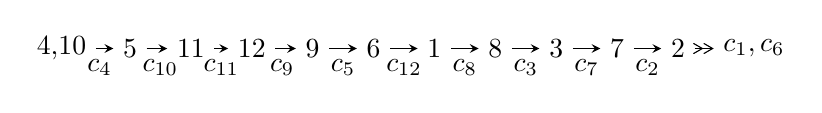
\begin{tikzpicture}[x=22pt, y=7pt]
	% node
	\node (A0) at (-1/8, 0) {4,10};
	\node (A1) at (1, 0) {5};
	\node (A2) at (2, 0) {11};
	\node (A3) at (3, 0) {12};
	\node (A4) at (4, 0) {9};
	\node (A5) at (5, 0) {6};
	\node (A6) at (6, 0) {1};
	\node (A7) at (7, 0) {8};
	\node (A8) at (8, 0) {3};
	\node (A9) at (9, 0) {7};
	\node (A10) at (10, 0) {2};
	\node (C1) at (1/2, -1) {$c_{4}$};
	\node (C2) at (3/2, -1) {$c_{10}$};
	\node (C3) at (5/2, -1) {$c_{11}$};
	\node (C4) at (7/2, -1) {$c_{9}$};
	\node (C5) at (9/2, -1) {$c_{5}$};
	\node (C6) at (11/2, -1) {$c_{12}$};
	\node (C7) at (13/2, -1) {$c_{8}$};
	\node (C8) at (15/2, -1) {$c_{3}$};
	\node (C9) at (17/2, -1) {$c_{7}$};
	\node (C10) at (19/2, -1) {$c_{2}$};
	\node (A11) at (45/4, 0) {$c_{1},c_{6}$};

	% edge
	\draw[->,>=stealth]	
	(A0) edge (A1) (A1) edge (A2) (A2) edge (A3) (A3) edge (A4) (A4) edge (A5) (A5) edge (A6) (A6) edge (A7) (A7) edge (A8) (A8) edge (A9) (A9) edge (A10) ;
	\draw[->>,>={angle 60}]	
	(A10) edge (A11);
\end{tikzpicture} \\ 

\end{tabular} \\

\footnotetext{
The image of knot diagram is generated by the software ``\textbf{Draw programme}" developed by Andrew Bartholomew(\url{http://www.layer8.co.uk/maths/draw/index.htm\#Running-draw}), where we modified some parts for our purpose(\url{https://github.com/CATsTAILs/LinksPainter}).
}\phantom \\ \newline 
\centering \textbf{Ideals for irreducible components\footnotemark of $X_{\text{par}}$} 
 
\begin{align*}
I^u_{1}&=\langle 
u^{90}+2 u^{89}+\cdots+3 u+1\rangle \\
I^u_{2}&=\langle 
u-1\rangle \\
\\
\end{align*}
\raggedright * 2 irreducible components of $\dim_{\mathbb{C}}=0$, with total 91 representations.\\
\footnotetext{All coefficients of polynomials are rational numbers. But the coefficients are sometimes approximated in decimal forms when there is not enough margin.}
\newpage
\renewcommand{\arraystretch}{1}
\centering \section*{I. $I^u_{1}= \langle u^{90}+2 u^{89}+\cdots+3 u+1 \rangle$}
\flushleft \textbf{(i) Arc colorings}\\
\begin{tabular}{m{7pt} m{180pt} m{7pt} m{180pt} }
\flushright $a_{4}=$&$\begin{pmatrix}1\\0\end{pmatrix}$ \\
\flushright $a_{10}=$&$\begin{pmatrix}0\\u\end{pmatrix}$ \\
\flushright $a_{5}=$&$\begin{pmatrix}1\\- u^2\end{pmatrix}$ \\
\flushright $a_{11}=$&$\begin{pmatrix}u\\- u^3+u\end{pmatrix}$ \\
\flushright $a_{12}=$&$\begin{pmatrix}u^3\\- u^3+u\end{pmatrix}$ \\
\flushright $a_{9}=$&$\begin{pmatrix}- u^3\\u^5- u^3+u\end{pmatrix}$ \\
\flushright $a_{6}=$&$\begin{pmatrix}u^6- u^4+1\\- u^8+2 u^6-2 u^4\end{pmatrix}$ \\
\flushright $a_{1}=$&$\begin{pmatrix}u^{17}-4 u^{15}+7 u^{13}-4 u^{11}-3 u^9+6 u^7-2 u^5+u\\- u^{19}+5 u^{17}-12 u^{15}+15 u^{13}-9 u^{11}- u^9+4 u^7-2 u^5- u^3+u\end{pmatrix}$ \\
\flushright $a_{8}=$&$\begin{pmatrix}- u^{11}+2 u^9-2 u^7- u^3\\u^{11}-3 u^9+4 u^7- u^5- u^3+u\end{pmatrix}$ \\
\flushright $a_{3}=$&$\begin{pmatrix}- u^{22}+5 u^{20}-12 u^{18}+15 u^{16}-10 u^{14}+2 u^{12}- u^8+u^6- u^4+1\\u^{22}-6 u^{20}+17 u^{18}-26 u^{16}+20 u^{14}-13 u^{10}+10 u^8- u^6-2 u^4+u^2\end{pmatrix}$ \\
\flushright $a_{7}=$&$\begin{pmatrix}u^{47}-12 u^{45}+\cdots+4 u^7-2 u^3\\- u^{49}+13 u^{47}+\cdots-2 u^3+u\end{pmatrix}$ \\
\flushright $a_{2}=$&$\begin{pmatrix}u^{63}-16 u^{61}+\cdots-6 u^7+2 u^3\\- u^{63}+17 u^{61}+\cdots-2 u^3+u\end{pmatrix}$\\&\end{tabular}
\flushleft \textbf{(ii) Obstruction class $= -1$}\\~\\
\flushleft \textbf{(iii) Cusp Shapes $= 4 u^{89}-96 u^{87}+\cdots+8 u-2$}\\~\\
\newpage\renewcommand{\arraystretch}{1}
\flushleft \textbf{(iv) u-Polynomials at the component}\newline \\
\begin{tabular}{m{50pt}|m{274pt}}
Crossings & \hspace{64pt}u-Polynomials at each crossing \\
\hline $$\begin{aligned}c_{1}\end{aligned}$$&$\begin{aligned}
&u^{90}+40 u^{89}+\cdots+u+1
\end{aligned}$\\
\hline $$\begin{aligned}c_{2},c_{6}\end{aligned}$$&$\begin{aligned}
&u^{90}-20 u^{88}+\cdots- u+1
\end{aligned}$\\
\hline $$\begin{aligned}c_{3},c_{12}\end{aligned}$$&$\begin{aligned}
&u^{90}+2 u^{89}+\cdots+35 u+25
\end{aligned}$\\
\hline $$\begin{aligned}c_{4},c_{10}\end{aligned}$$&$\begin{aligned}
&u^{90}+2 u^{89}+\cdots+3 u+1
\end{aligned}$\\
\hline $$\begin{aligned}c_{5},c_{11}\end{aligned}$$&$\begin{aligned}
&u^{90}+3 u^{89}+\cdots-37 u+13
\end{aligned}$\\
\hline $$\begin{aligned}c_{7}\end{aligned}$$&$\begin{aligned}
&u^{90}-3 u^{89}+\cdots-69 u+13
\end{aligned}$\\
\hline $$\begin{aligned}c_{8}\end{aligned}$$&$\begin{aligned}
&u^{90}+14 u^{89}+\cdots+26531 u+1493
\end{aligned}$\\
\hline $$\begin{aligned}c_{9}\end{aligned}$$&$\begin{aligned}
&u^{90}-48 u^{89}+\cdots- u+1
\end{aligned}$\\
\hline
\end{tabular}\\~\\
\newpage\renewcommand{\arraystretch}{1}
\flushleft \textbf{(v) Riley Polynomials at the component}\newline \\
\begin{tabular}{m{50pt}|m{274pt}}
Crossings & \hspace{64pt}Riley Polynomials at each crossing \\
\hline $$\begin{aligned}c_{1}\end{aligned}$$&$\begin{aligned}
&y^{90}+20 y^{89}+\cdots-5 y+1
\end{aligned}$\\
\hline $$\begin{aligned}c_{2},c_{6}\end{aligned}$$&$\begin{aligned}
&y^{90}-40 y^{89}+\cdots- y+1
\end{aligned}$\\
\hline $$\begin{aligned}c_{3},c_{12}\end{aligned}$$&$\begin{aligned}
&y^{90}-72 y^{89}+\cdots+675 y+625
\end{aligned}$\\
\hline $$\begin{aligned}c_{4},c_{10}\end{aligned}$$&$\begin{aligned}
&y^{90}-48 y^{89}+\cdots- y+1
\end{aligned}$\\
\hline $$\begin{aligned}c_{5},c_{11}\end{aligned}$$&$\begin{aligned}
&y^{90}+75 y^{89}+\cdots-21571 y+169
\end{aligned}$\\
\hline $$\begin{aligned}c_{7}\end{aligned}$$&$\begin{aligned}
&y^{90}+3 y^{89}+\cdots+8941 y+169
\end{aligned}$\\
\hline $$\begin{aligned}c_{8}\end{aligned}$$&$\begin{aligned}
&y^{90}-24 y^{89}+\cdots-76057601 y+2229049
\end{aligned}$\\
\hline $$\begin{aligned}c_{9}\end{aligned}$$&$\begin{aligned}
&y^{90}-12 y^{89}+\cdots+3 y+1
\end{aligned}$\\
\hline
\end{tabular}\\~\\
\newpage\flushleft \textbf{(vi) Complex Volumes and Cusp Shapes}
$$\begin{array}{c|c|c}  
\text{Solutions to }I^u_{1}& \I (\text{vol} + \sqrt{-1}CS) & \text{Cusp shape}\\
 \hline 
\begin{aligned}
u &= -0.873411 + 0.513697 I\end{aligned}
 & -1.81913 - 4.09974 I & \phantom{-0.000000 } 0 \\ \hline\begin{aligned}
u &= -0.873411 - 0.513697 I\end{aligned}
 & -1.81913 + 4.09974 I & \phantom{-0.000000 } 0 \\ \hline\begin{aligned}
u &= \phantom{-}0.902181 + 0.525801 I\end{aligned}
 & \phantom{-}2.99810 + 6.09081 I & \phantom{-0.000000 } 0 \\ \hline\begin{aligned}
u &= \phantom{-}0.902181 - 0.525801 I\end{aligned}
 & \phantom{-}2.99810 - 6.09081 I & \phantom{-0.000000 } 0 \\ \hline\begin{aligned}
u &= -0.897963 + 0.536251 I\end{aligned}
 & \phantom{-}1.02275 - 11.20450 I & \phantom{-0.000000 } 0 \\ \hline\begin{aligned}
u &= -0.897963 - 0.536251 I\end{aligned}
 & \phantom{-}1.02275 + 11.20450 I & \phantom{-0.000000 } 0 \\ \hline\begin{aligned}
u &= \phantom{-}0.922566 + 0.496402 I\end{aligned}
 & \phantom{-}3.48059 + 3.55498 I & \phantom{-0.000000 } 0 \\ \hline\begin{aligned}
u &= \phantom{-}0.922566 - 0.496402 I\end{aligned}
 & \phantom{-}3.48059 - 3.55498 I & \phantom{-0.000000 } 0 \\ \hline\begin{aligned}
u &= -0.903572 + 0.276220 I\end{aligned}
 & \phantom{-}0.20740 - 3.77187 I & \phantom{-}5.01166 + 7.48596 I \\ \hline\begin{aligned}
u &= -0.903572 - 0.276220 I\end{aligned}
 & \phantom{-}0.20740 + 3.77187 I & \phantom{-}5.01166 - 7.48596 I \\ \hline\begin{aligned}
u &= \phantom{-}0.788143 + 0.520655 I\end{aligned}
 & -4.28906 + 5.70288 I & -4.46481 - 8.34300 I \\ \hline\begin{aligned}
u &= \phantom{-}0.788143 - 0.520655 I\end{aligned}
 & -4.28906 - 5.70288 I & -4.46481 + 8.34300 I \\ \hline\begin{aligned}
u &= -0.941169 + 0.480866 I\end{aligned}
 & \phantom{-}1.91087 + 1.41955 I & \phantom{-0.000000 } 0 \\ \hline\begin{aligned}
u &= -0.941169 - 0.480866 I\end{aligned}
 & \phantom{-}1.91087 - 1.41955 I & \phantom{-0.000000 } 0 \\ \hline\begin{aligned}
u &= -1.059210 + 0.019229 I\end{aligned}
 & \phantom{-}6.75320 - 1.38707 I & \phantom{-0.000000 } 0 \\ \hline\begin{aligned}
u &= -1.059210 - 0.019229 I\end{aligned}
 & \phantom{-}6.75320 + 1.38707 I & \phantom{-0.000000 } 0 \\ \hline\begin{aligned}
u &= \phantom{-}1.063040 + 0.035242 I\end{aligned}
 & \phantom{-}4.97510 + 6.54466 I & \phantom{-0.000000 } 0 \\ \hline\begin{aligned}
u &= \phantom{-}1.063040 - 0.035242 I\end{aligned}
 & \phantom{-}4.97510 - 6.54466 I & \phantom{-0.000000 } 0 \\ \hline\begin{aligned}
u &= -0.770968 + 0.482215 I\end{aligned}
 & -1.57766 - 2.01209 I & -0.85760 + 4.47164 I \\ \hline\begin{aligned}
u &= -0.770968 - 0.482215 I\end{aligned}
 & -1.57766 + 2.01209 I & -0.85760 - 4.47164 I \\ \hline\begin{aligned}
u &= \phantom{-}0.738456 + 0.517645 I\end{aligned}
 & -4.43144 - 1.45967 I & -5.28174 + 0.47374 I \\ \hline\begin{aligned}
u &= \phantom{-}0.738456 - 0.517645 I\end{aligned}
 & -4.43144 + 1.45967 I & -5.28174 - 0.47374 I \\ \hline\begin{aligned}
u &= \phantom{-}0.831064 + 0.096380 I\end{aligned}
 & \phantom{-}1.270970 + 0.122716 I & \phantom{-}8.82726 - 0.42041 I \\ \hline\begin{aligned}
u &= \phantom{-}0.831064 - 0.096380 I\end{aligned}
 & \phantom{-}1.270970 - 0.122716 I & \phantom{-}8.82726 + 0.42041 I \\ \hline\begin{aligned}
u &= -0.126989 + 0.822033 I\end{aligned}
 & \phantom{-}4.77347 + 11.44800 I & \phantom{-}3.37132 - 7.61382 I \\ \hline\begin{aligned}
u &= -0.126989 - 0.822033 I\end{aligned}
 & \phantom{-}4.77347 - 11.44800 I & \phantom{-}3.37132 + 7.61382 I \\ \hline\begin{aligned}
u &= \phantom{-}0.120864 + 0.820667 I\end{aligned}
 & \phantom{-}6.74638 - 6.20589 I & \phantom{-}6.36909 + 3.29581 I \\ \hline\begin{aligned}
u &= \phantom{-}0.120864 - 0.820667 I\end{aligned}
 & \phantom{-}6.74638 + 6.20589 I & \phantom{-}6.36909 - 3.29581 I \\ \hline\begin{aligned}
u &= \phantom{-}0.103336 + 0.819213 I\end{aligned}
 & \phantom{-}7.26934 - 3.28559 I & \phantom{-}7.18981 + 2.93019 I \\ \hline\begin{aligned}
u &= \phantom{-}0.103336 - 0.819213 I\end{aligned}
 & \phantom{-}7.26934 + 3.28559 I & \phantom{-}7.18981 - 2.93019 I\\
 \hline 
 \end{array}$$\newpage$$\begin{array}{c|c|c}  
\text{Solutions to }I^u_{1}& \I (\text{vol} + \sqrt{-1}CS) & \text{Cusp shape}\\
 \hline 
\begin{aligned}
u &= -0.094198 + 0.819093 I\end{aligned}
 & \phantom{-}5.74525 - 1.91608 I & \phantom{-}4.94203 + 2.18879 I \\ \hline\begin{aligned}
u &= -0.094198 - 0.819093 I\end{aligned}
 & \phantom{-}5.74525 + 1.91608 I & \phantom{-}4.94203 - 2.18879 I \\ \hline\begin{aligned}
u &= -0.120401 + 0.803953 I\end{aligned}
 & \phantom{-}1.59070 + 4.18357 I & \phantom{-}0.16117 - 3.00795 I \\ \hline\begin{aligned}
u &= -0.120401 - 0.803953 I\end{aligned}
 & \phantom{-}1.59070 - 4.18357 I & \phantom{-}0.16117 + 3.00795 I \\ \hline\begin{aligned}
u &= -0.578569 + 0.559212 I\end{aligned}
 & \phantom{-}0.13368 + 6.80952 I & -0.27186 - 4.68036 I \\ \hline\begin{aligned}
u &= -0.578569 - 0.559212 I\end{aligned}
 & \phantom{-}0.13368 - 6.80952 I & -0.27186 + 4.68036 I \\ \hline\begin{aligned}
u &= -0.620498 + 0.503672 I\end{aligned}
 & -2.52931 - 0.09500 I & -4.25506 + 0.72855 I \\ \hline\begin{aligned}
u &= -0.620498 - 0.503672 I\end{aligned}
 & -2.52931 + 0.09500 I & -4.25506 - 0.72855 I \\ \hline\begin{aligned}
u &= -1.130970 + 0.433801 I\end{aligned}
 & \phantom{-}0.70255 - 4.46851 I & \phantom{-0.000000 } 0 \\ \hline\begin{aligned}
u &= -1.130970 - 0.433801 I\end{aligned}
 & \phantom{-}0.70255 + 4.46851 I & \phantom{-0.000000 } 0 \\ \hline\begin{aligned}
u &= -1.152640 + 0.389106 I\end{aligned}
 & \phantom{-}1.84992 + 2.50588 I & \phantom{-0.000000 } 0 \\ \hline\begin{aligned}
u &= -1.152640 - 0.389106 I\end{aligned}
 & \phantom{-}1.84992 - 2.50588 I & \phantom{-0.000000 } 0 \\ \hline\begin{aligned}
u &= \phantom{-}0.561042 + 0.544183 I\end{aligned}
 & \phantom{-}2.05754 - 1.76920 I & \phantom{-}2.90604 + 0.28243 I \\ \hline\begin{aligned}
u &= \phantom{-}0.561042 - 0.544183 I\end{aligned}
 & \phantom{-}2.05754 + 1.76920 I & \phantom{-}2.90604 - 0.28243 I \\ \hline\begin{aligned}
u &= \phantom{-}1.162250 + 0.412550 I\end{aligned}
 & \phantom{-}4.17297 + 1.71901 I & \phantom{-0.000000 } 0 \\ \hline\begin{aligned}
u &= \phantom{-}1.162250 - 0.412550 I\end{aligned}
 & \phantom{-}4.17297 - 1.71901 I & \phantom{-0.000000 } 0 \\ \hline\begin{aligned}
u &= -0.024292 + 0.753892 I\end{aligned}
 & \phantom{-}2.47216 + 2.13571 I & \phantom{-}5.91843 - 3.73421 I \\ \hline\begin{aligned}
u &= -0.024292 - 0.753892 I\end{aligned}
 & \phantom{-}2.47216 - 2.13571 I & \phantom{-}5.91843 + 3.73421 I \\ \hline\begin{aligned}
u &= \phantom{-}1.152150 + 0.484969 I\end{aligned}
 & \phantom{-}0.27112 + 3.48997 I & \phantom{-0.000000 } 0 \\ \hline\begin{aligned}
u &= \phantom{-}1.152150 - 0.484969 I\end{aligned}
 & \phantom{-}0.27112 - 3.48997 I & \phantom{-0.000000 } 0 \\ \hline\begin{aligned}
u &= \phantom{-}0.153502 + 0.729188 I\end{aligned}
 & -1.85254 - 6.16807 I & -1.72016 + 7.05399 I \\ \hline\begin{aligned}
u &= \phantom{-}0.153502 - 0.729188 I\end{aligned}
 & -1.85254 + 6.16807 I & -1.72016 - 7.05399 I \\ \hline\begin{aligned}
u &= -1.170070 + 0.486533 I\end{aligned}
 & \phantom{-}3.64084 - 6.60935 I & \phantom{-0.000000 } 0 \\ \hline\begin{aligned}
u &= -1.170070 - 0.486533 I\end{aligned}
 & \phantom{-}3.64084 + 6.60935 I & \phantom{-0.000000 } 0 \\ \hline\begin{aligned}
u &= \phantom{-}1.167280 + 0.498284 I\end{aligned}
 & \phantom{-}1.08161 + 10.76960 I & \phantom{-0.000000 } 0 \\ \hline\begin{aligned}
u &= \phantom{-}1.167280 - 0.498284 I\end{aligned}
 & \phantom{-}1.08161 - 10.76960 I & \phantom{-0.000000 } 0 \\ \hline\begin{aligned}
u &= \phantom{-}1.191320 + 0.443194 I\end{aligned}
 & \phantom{-}5.96752 + 2.13257 I & \phantom{-0.000000 } 0 \\ \hline\begin{aligned}
u &= \phantom{-}1.191320 - 0.443194 I\end{aligned}
 & \phantom{-}5.96752 - 2.13257 I & \phantom{-0.000000 } 0 \\ \hline\begin{aligned}
u &= \phantom{-}1.213250 + 0.391111 I\end{aligned}
 & \phantom{-}5.57380 - 0.11285 I & \phantom{-0.000000 } 0 \\ \hline\begin{aligned}
u &= \phantom{-}1.213250 - 0.391111 I\end{aligned}
 & \phantom{-}5.57380 + 0.11285 I & \phantom{-0.000000 } 0\\
 \hline 
 \end{array}$$\newpage$$\begin{array}{c|c|c}  
\text{Solutions to }I^u_{1}& \I (\text{vol} + \sqrt{-1}CS) & \text{Cusp shape}\\
 \hline 
\begin{aligned}
u &= -0.116850 + 0.712914 I\end{aligned}
 & \phantom{-}0.62172 + 2.11128 I & \phantom{-}2.36589 - 3.42722 I \\ \hline\begin{aligned}
u &= -0.116850 - 0.712914 I\end{aligned}
 & \phantom{-}0.62172 - 2.11128 I & \phantom{-}2.36589 + 3.42722 I \\ \hline\begin{aligned}
u &= -1.191720 + 0.461019 I\end{aligned}
 & \phantom{-}5.84080 - 6.54472 I & \phantom{-0.000000 } 0 \\ \hline\begin{aligned}
u &= -1.191720 - 0.461019 I\end{aligned}
 & \phantom{-}5.84080 + 6.54472 I & \phantom{-0.000000 } 0 \\ \hline\begin{aligned}
u &= \phantom{-}0.485978 + 0.528952 I\end{aligned}
 & \phantom{-}2.30152 + 0.59676 I & \phantom{-}3.38135 - 0.44638 I \\ \hline\begin{aligned}
u &= \phantom{-}0.485978 - 0.528952 I\end{aligned}
 & \phantom{-}2.30152 - 0.59676 I & \phantom{-}3.38135 + 0.44638 I \\ \hline\begin{aligned}
u &= \phantom{-}1.224080 + 0.384721 I\end{aligned}
 & \phantom{-}8.85923 - 7.34311 I & \phantom{-0.000000 } 0 \\ \hline\begin{aligned}
u &= \phantom{-}1.224080 - 0.384721 I\end{aligned}
 & \phantom{-}8.85923 + 7.34311 I & \phantom{-0.000000 } 0 \\ \hline\begin{aligned}
u &= -1.223690 + 0.388798 I\end{aligned}
 & \phantom{-}10.80400 + 2.07981 I & \phantom{-0.000000 } 0 \\ \hline\begin{aligned}
u &= -1.223690 - 0.388798 I\end{aligned}
 & \phantom{-}10.80400 - 2.07981 I & \phantom{-0.000000 } 0 \\ \hline\begin{aligned}
u &= -1.223810 + 0.399626 I\end{aligned}
 & \phantom{-}11.25850 - 0.90671 I & \phantom{-0.000000 } 0 \\ \hline\begin{aligned}
u &= -1.223810 - 0.399626 I\end{aligned}
 & \phantom{-}11.25850 + 0.90671 I & \phantom{-0.000000 } 0 \\ \hline\begin{aligned}
u &= \phantom{-}1.224080 + 0.404848 I\end{aligned}
 & \phantom{-}9.70226 + 6.14308 I & \phantom{-0.000000 } 0 \\ \hline\begin{aligned}
u &= \phantom{-}1.224080 - 0.404848 I\end{aligned}
 & \phantom{-}9.70226 - 6.14308 I & \phantom{-0.000000 } 0 \\ \hline\begin{aligned}
u &= -0.450612 + 0.548105 I\end{aligned}
 & \phantom{-}0.55266 - 5.54561 I & \phantom{-}0.22267 + 5.35237 I \\ \hline\begin{aligned}
u &= -0.450612 - 0.548105 I\end{aligned}
 & \phantom{-}0.55266 + 5.54561 I & \phantom{-}0.22267 - 5.35237 I \\ \hline\begin{aligned}
u &= -1.197770 + 0.505207 I\end{aligned}
 & \phantom{-}4.76470 - 8.98285 I & \phantom{-0.000000 } 0 \\ \hline\begin{aligned}
u &= -1.197770 - 0.505207 I\end{aligned}
 & \phantom{-}4.76470 + 8.98285 I & \phantom{-0.000000 } 0 \\ \hline\begin{aligned}
u &= -1.208040 + 0.497568 I\end{aligned}
 & \phantom{-}9.04174 - 2.87641 I & \phantom{-0.000000 } 0 \\ \hline\begin{aligned}
u &= -1.208040 - 0.497568 I\end{aligned}
 & \phantom{-}9.04174 + 2.87641 I & \phantom{-0.000000 } 0 \\ \hline\begin{aligned}
u &= \phantom{-}1.206570 + 0.501359 I\end{aligned}
 & \phantom{-}10.53440 + 8.09975 I & \phantom{-0.000000 } 0 \\ \hline\begin{aligned}
u &= \phantom{-}1.206570 - 0.501359 I\end{aligned}
 & \phantom{-}10.53440 - 8.09975 I & \phantom{-0.000000 } 0 \\ \hline\begin{aligned}
u &= \phantom{-}1.203810 + 0.508612 I\end{aligned}
 & \phantom{-}9.9530 + 11.0635 I & \phantom{-0.000000 } 0 \\ \hline\begin{aligned}
u &= \phantom{-}1.203810 - 0.508612 I\end{aligned}
 & \phantom{-}9.9530 - 11.0635 I & \phantom{-0.000000 } 0 \\ \hline\begin{aligned}
u &= -1.203080 + 0.511255 I\end{aligned}
 & \phantom{-}7.9613 - 16.3232 I & \phantom{-0.000000 } 0 \\ \hline\begin{aligned}
u &= -1.203080 - 0.511255 I\end{aligned}
 & \phantom{-}7.9613 + 16.3232 I & \phantom{-0.000000 } 0 \\ \hline\begin{aligned}
u &= \phantom{-}0.164684 + 0.661302 I\end{aligned}
 & -2.55538 + 0.91259 I & -3.81773 - 0.78733 I \\ \hline\begin{aligned}
u &= \phantom{-}0.164684 - 0.661302 I\end{aligned}
 & -2.55538 - 0.91259 I & -3.81773 + 0.78733 I \\ \hline\begin{aligned}
u &= -0.299147 + 0.470065 I\end{aligned}
 & -1.76511 + 0.79975 I & -3.82418 - 0.77073 I \\ \hline\begin{aligned}
u &= -0.299147 - 0.470065 I\end{aligned}
 & -1.76511 - 0.79975 I & -3.82418 + 0.77073 I\\
 \hline 
 \end{array}$$\newpage\newpage\renewcommand{\arraystretch}{1}
\centering \section*{II. $I^u_{2}= \langle u-1 \rangle$}
\flushleft \textbf{(i) Arc colorings}\\
\begin{tabular}{m{7pt} m{180pt} m{7pt} m{180pt} }
\flushright $a_{4}=$&$\begin{pmatrix}1\\0\end{pmatrix}$ \\
\flushright $a_{10}=$&$\begin{pmatrix}0\\1\end{pmatrix}$ \\
\flushright $a_{5}=$&$\begin{pmatrix}1\\-1\end{pmatrix}$ \\
\flushright $a_{11}=$&$\begin{pmatrix}1\\0\end{pmatrix}$ \\
\flushright $a_{12}=$&$\begin{pmatrix}1\\0\end{pmatrix}$ \\
\flushright $a_{9}=$&$\begin{pmatrix}-1\\1\end{pmatrix}$ \\
\flushright $a_{6}=$&$\begin{pmatrix}1\\-1\end{pmatrix}$ \\
\flushright $a_{1}=$&$\begin{pmatrix}2\\-1\end{pmatrix}$ \\
\flushright $a_{8}=$&$\begin{pmatrix}-2\\1\end{pmatrix}$ \\
\flushright $a_{3}=$&$\begin{pmatrix}-1\\1\end{pmatrix}$ \\
\flushright $a_{7}=$&$\begin{pmatrix}-2\\1\end{pmatrix}$ \\
\flushright $a_{2}=$&$\begin{pmatrix}1\\0\end{pmatrix}$\\&\end{tabular}
\flushleft \textbf{(ii) Obstruction class $= -1$}\\~\\
\flushleft \textbf{(iii) Cusp Shapes $= 6$}\\~\\
\newpage\renewcommand{\arraystretch}{1}
\flushleft \textbf{(iv) u-Polynomials at the component}\newline \\
\begin{tabular}{m{50pt}|m{274pt}}
Crossings & \hspace{64pt}u-Polynomials at each crossing \\
\hline $$\begin{aligned}c_{1}\end{aligned}$$&$\begin{aligned}
&u+1
\end{aligned}$\\
\hline $$\begin{aligned}c_{2},c_{3},c_{4}\\c_{6},c_{8},c_{9}\\c_{10},c_{12}\end{aligned}$$&$\begin{aligned}
&u-1
\end{aligned}$\\
\hline $$\begin{aligned}c_{5},c_{7},c_{11}\end{aligned}$$&$\begin{aligned}
&u
\end{aligned}$\\
\hline
\end{tabular}\\~\\
\newpage\renewcommand{\arraystretch}{1}
\flushleft \textbf{(v) Riley Polynomials at the component}\newline \\
\begin{tabular}{m{50pt}|m{274pt}}
Crossings & \hspace{64pt}Riley Polynomials at each crossing \\
\hline $$\begin{aligned}c_{1},c_{2},c_{3}\\c_{4},c_{6},c_{8}\\c_{9},c_{10},c_{12}\end{aligned}$$&$\begin{aligned}
&y-1
\end{aligned}$\\
\hline $$\begin{aligned}c_{5},c_{7},c_{11}\end{aligned}$$&$\begin{aligned}
&y
\end{aligned}$\\
\hline
\end{tabular}\\~\\
\newpage\flushleft \textbf{(vi) Complex Volumes and Cusp Shapes}
$$\begin{array}{c|c|c}  
\text{Solutions to }I^u_{2}& \I (\text{vol} + \sqrt{-1}CS) & \text{Cusp shape}\\
 \hline 
\begin{aligned}
u &= \phantom{-}1.00000\phantom{ +0.000000I}\end{aligned}
 & \phantom{-}1.64493\phantom{ +0.000000I} & \phantom{-}6.00000\phantom{ +0.000000I}\\
 \hline 
 \end{array}$$\newpage
\newpage\renewcommand{\arraystretch}{1}
\centering \section*{ III. u-Polynomials}
\begin{tabular}{m{50pt}|m{274pt}}
Crossings & \hspace{64pt}u-Polynomials at each crossing \\
\hline $$\begin{aligned}c_{1}\end{aligned}$$&$\begin{aligned}
&(u+1)(u^{90}+40 u^{89}+\cdots+u+1)
\end{aligned}$\\
\hline $$\begin{aligned}c_{2},c_{6}\end{aligned}$$&$\begin{aligned}
&(u-1)(u^{90}-20 u^{88}+\cdots- u+1)
\end{aligned}$\\
\hline $$\begin{aligned}c_{3},c_{12}\end{aligned}$$&$\begin{aligned}
&(u-1)(u^{90}+2 u^{89}+\cdots+35 u+25)
\end{aligned}$\\
\hline $$\begin{aligned}c_{4},c_{10}\end{aligned}$$&$\begin{aligned}
&(u-1)(u^{90}+2 u^{89}+\cdots+3 u+1)
\end{aligned}$\\
\hline $$\begin{aligned}c_{5},c_{11}\end{aligned}$$&$\begin{aligned}
&u(u^{90}+3 u^{89}+\cdots-37 u+13)
\end{aligned}$\\
\hline $$\begin{aligned}c_{7}\end{aligned}$$&$\begin{aligned}
&u(u^{90}-3 u^{89}+\cdots-69 u+13)
\end{aligned}$\\
\hline $$\begin{aligned}c_{8}\end{aligned}$$&$\begin{aligned}
&(u-1)(u^{90}+14 u^{89}+\cdots+26531 u+1493)
\end{aligned}$\\
\hline $$\begin{aligned}c_{9}\end{aligned}$$&$\begin{aligned}
&(u-1)(u^{90}-48 u^{89}+\cdots- u+1)
\end{aligned}$\\
\hline
\end{tabular}\newpage\renewcommand{\arraystretch}{1}
\centering \section*{ IV. Riley Polynomials}
\begin{tabular}{m{50pt}|m{274pt}}
Crossings & \hspace{64pt}Riley Polynomials at each crossing \\
\hline $$\begin{aligned}c_{1}\end{aligned}$$&$\begin{aligned}
&(y-1)(y^{90}+20 y^{89}+\cdots-5 y+1)
\end{aligned}$\\
\hline $$\begin{aligned}c_{2},c_{6}\end{aligned}$$&$\begin{aligned}
&(y-1)(y^{90}-40 y^{89}+\cdots- y+1)
\end{aligned}$\\
\hline $$\begin{aligned}c_{3},c_{12}\end{aligned}$$&$\begin{aligned}
&(y-1)(y^{90}-72 y^{89}+\cdots+675 y+625)
\end{aligned}$\\
\hline $$\begin{aligned}c_{4},c_{10}\end{aligned}$$&$\begin{aligned}
&(y-1)(y^{90}-48 y^{89}+\cdots- y+1)
\end{aligned}$\\
\hline $$\begin{aligned}c_{5},c_{11}\end{aligned}$$&$\begin{aligned}
&y(y^{90}+75 y^{89}+\cdots-21571 y+169)
\end{aligned}$\\
\hline $$\begin{aligned}c_{7}\end{aligned}$$&$\begin{aligned}
&y(y^{90}+3 y^{89}+\cdots+8941 y+169)
\end{aligned}$\\
\hline $$\begin{aligned}c_{8}\end{aligned}$$&$\begin{aligned}
&(y-1)(y^{90}-24 y^{89}+\cdots-7.60576\times10^{7} y+2229049)
\end{aligned}$\\
\hline $$\begin{aligned}c_{9}\end{aligned}$$&$\begin{aligned}
&(y-1)(y^{90}-12 y^{89}+\cdots+3 y+1)
\end{aligned}$\\
\hline
\end{tabular}
\vskip 2pc
\end{document}